\textbf{Цель: }Получить навыки формализации и обработки информации с
использованием семантических сетей

\textbf{Задача: }Поиск одного из минимальных путей между двумя вершинами
в неориентированном графе

\section{Список понятий}

\begin{enumerate}
\item
  Графовая структура (абсолютное понятие) - это такая одноуровневая
  реляционная структура, объекты которой могут играть роль либо вершины,
  либо связки:

  \begin{enumerate}
  \item
    Вершина (относительное понятие, ролевое отношение);
  \item
    Связка (относительное понятие, ролевое отношение).
  \end{enumerate}

\begin{figure}[H]
  \centering
  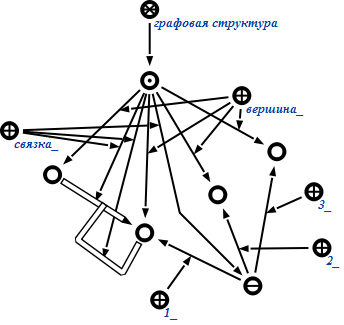
\includegraphics[scale=0.7]{images/1.png}
  \caption{Графовая структура}
\end{figure}

\item
  Графовая структура с ориентированными связками (абсолютное понятие)

  \begin{enumerate}
  \item
    Ориентированная связка (относительное понятие, ролевое отношение)
    -- связка, которая задается ориентированным множеством.
  \end{enumerate}

\begin{figure}[H]
  \centering
  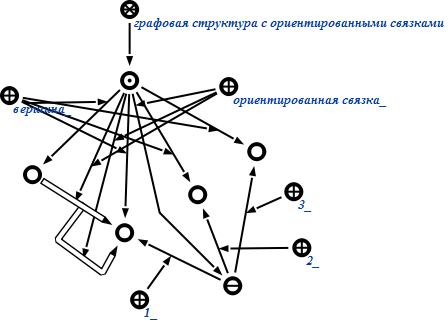
\includegraphics[scale=0.7]{images/2.png}
  \caption{Графовая структура с ориентированными связками}
\end{figure}

\item
  Графовая структура с неориентированными связками (абсолютное понятие)

  \begin{enumerate}
  \item
    Неориентированная связка (относительное понятие, ролевое отношение)
    --связка, которая задается неориентированным множеством.
  \end{enumerate}

\begin{figure}[H]
  \centering
  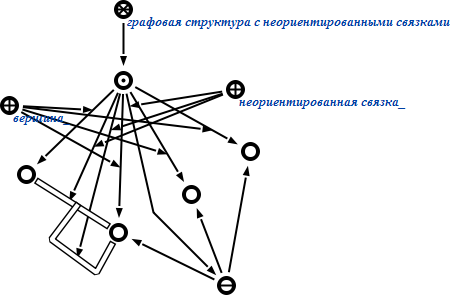
\includegraphics[scale=0.7]{images/3.png}
  \caption{Графовая структура с неориентированными связками}
\end{figure}

\item
  Гиперграф (абсолютное понятие) -- это такая графовая структура, в
  которой связки могут связывать только вершины:

  \begin{enumerate}
  \item
    Гиперсвязка (относительное понятие, ролевое отношение);
  \item
    Гипердуга (относительное понятие, ролевое отношение) --
    ориентированнаягиперсвязка;
  \item
    Гиперребро (относительное понятие, ролевое отношение) --
    неориентированнаягиперсвязка.
  \end{enumerate}

\begin{figure}[H]
  \centering
  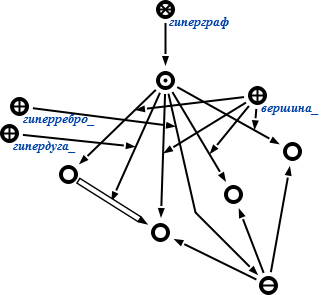
\includegraphics[scale=0.7]{images/4.png}
  \caption{Гиперграф}
\end{figure}

\item
  Псевдограф (абсолютное понятие) -- это такой гиперграф, в котором все
  связки должны быть бинарными:

  \begin{enumerate}
  \item
    Бинарная связка (относительное понятие, ролевое отношение)
    --гиперсвязка арности 2;
  \item
    Ребро (относительное понятие, ролевое отношение)
    --неориентированнаягиперсвязка;
  \item
    Дуга (относительное понятие, ролевое отношение) -- ориентированная
    гиперсвязка;
  \item
    Петля (относительное понятие, ролевое отношение) -- бинарная связка,
    у которой первый и второй компоненты совпадают.
  \end{enumerate}

\begin{figure}[H]
  \centering
  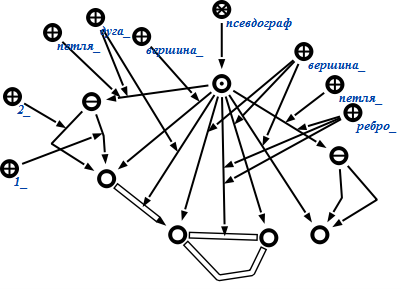
\includegraphics[scale=0.7]{images/5.png}
  \caption{Псевдограф}
\end{figure}

\item
  Мультиграф (абсолютное понятие) -- это такой псевдограф, в котором не
  может быть петель:

\begin{figure}[H]
  \centering
  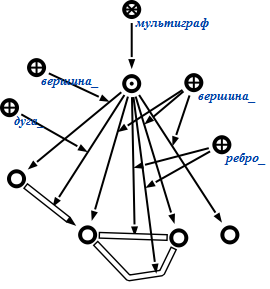
\includegraphics[scale=0.7]{images/6.png}
  \caption{Мультиграф}
\end{figure}

\item
  Граф (абсолютное понятие) -- это такой мультиграф, в котором не может
  быть кратных связок, т.е. связок у которых первый и второй компоненты
  совпадают:

\begin{figure}[H]
  \centering
  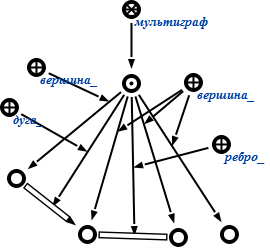
\includegraphics[scale=0.7]{images/7.png}
  \caption{Граф}
\end{figure}

\item
  Неориентированный граф (абсолютное понятие) --это такой граф, в
  котором все связки являются ребрами:

\begin{figure}[H]
  \centering
  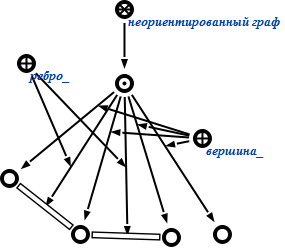
\includegraphics[scale=0.7]{images/8.png}
  \caption{Неориентированный граф}
\end{figure}

\item
  Ориентированный граф (абсолютное понятие) - это такой граф, в котором
  все связки являются дугами:

\begin{figure}[H]
  \centering
  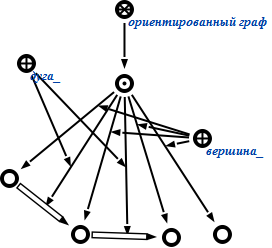
\includegraphics[scale=0.7]{images/9.png}
  \caption{Ориентированный граф}
\end{figure}

\item
  Маршрут (относительное понятие, бинарное ориентированное отношение) --
  это чередующаяся последовательность вершин и гиперсвязок в гиперграфе,
  которая начинается и кончается вершиной, и каждая гиперсвязка
  последовательности инцидентна двум вершинам, одна из которых
  непосредственно предшествует ей, а другая непосредственно следует за
  ней. В примере ниже показан маршрут \emph{A}, \emph{CON1}, \emph{C},
  \emph{CON2}, \emph{D}, \emph{CON3}, \emph{B}, \emph{CON1}, \emph{A} в
  гиперграфе.

\begin{figure}[H]
  \centering
  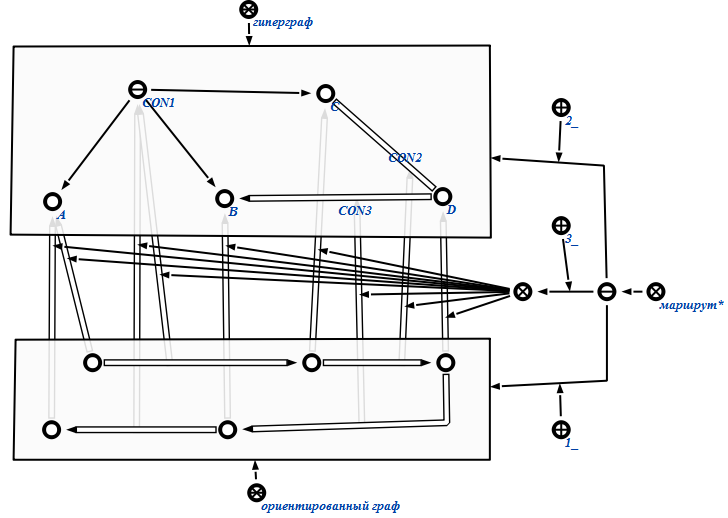
\includegraphics[scale=0.7]{images/10.png}
  \caption{Маршрут}
\end{figure}

\item
  Цепь (относительное понятие, бинарное ориентированное отношение) --
  это маршрут, все гиперсвязки которого различны. В примере ниже
  показана цепь \emph{A}, \emph{CON1}, \emph{C}, \emph{CON2}, \emph{D},
  \emph{CON3}, \emph{B}, \emph{CON4}, \emph{A} в гиперграфе.

\begin{figure}[H]
  \centering
  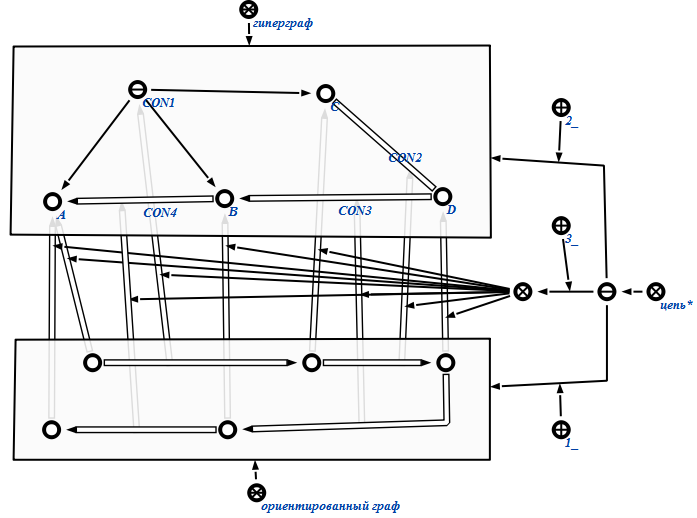
\includegraphics[scale=0.7]{images/11.png}
  \caption{Цепь}
\end{figure}

\item
  Простая цепь, путь (относительное понятие, бинарное ориентированное
  отношение) -- это цепь, в которой все вершины различны. В примере ниже
  показан путь \emph{A}, \emph{CON1}, \emph{C}, \emph{CON2}, \emph{D},
  \emph{CON3}, \emph{B} в гиперграфе.

\begin{figure}[H]
  \centering
  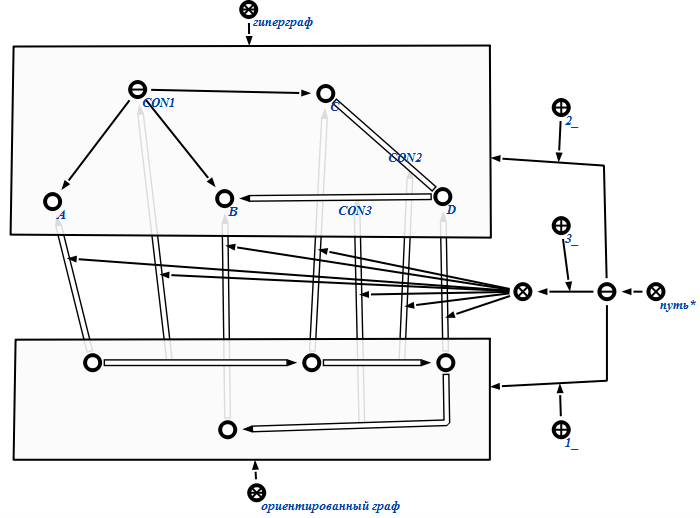
\includegraphics[scale=0.7]{images/12.png}
  \caption{Простая цепь}
\end{figure}

\end{enumerate}

\section{Тестовые примеры}

Во всех тестах графы будет приведены в сокращенной форме со скрытыми ролями элементов графа.

\subsection{Тест 1}

\textbf{Вход:}

Необходимо найти минимальный путь между вершинами A и C.

\begin{figure}[H]
  \centering
  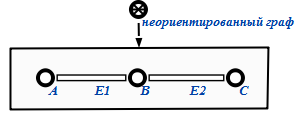
\includegraphics[scale=0.7]{images/13.png}
  \caption{Вход теста 1}
\end{figure}

\textbf{Выход:}

Будет найден единственный минимальный путь \emph{A}, \emph{E1},
\emph{B}, \emph{E2}, \emph{C}:

\begin{figure}[H]
  \centering
  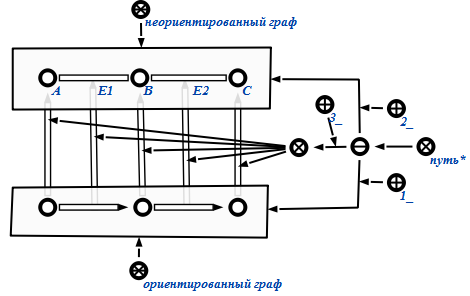
\includegraphics[scale=0.7]{images/14.png}
  \caption{Выход теста 1}
\end{figure}

\subsection{Тест 2}

\textbf{Вход:}

Необходимо найти минимальный путь между вершинами \emph{A} и \emph{F}.

\begin{figure}[H]
  \centering
  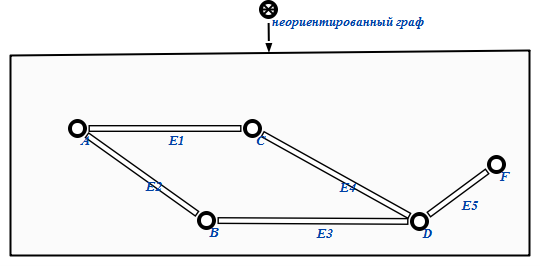
\includegraphics[scale=0.7]{images/15.png}
  \caption{Вход теста 2}
\end{figure}

\textbf{Выход:}

Будет найден один из двух минимальный путь \emph{A}, \emph{E2},
\emph{B}, \emph{E3}, \emph{D}, \emph{E5}, \emph{F}:

\begin{figure}[H]
  \centering
  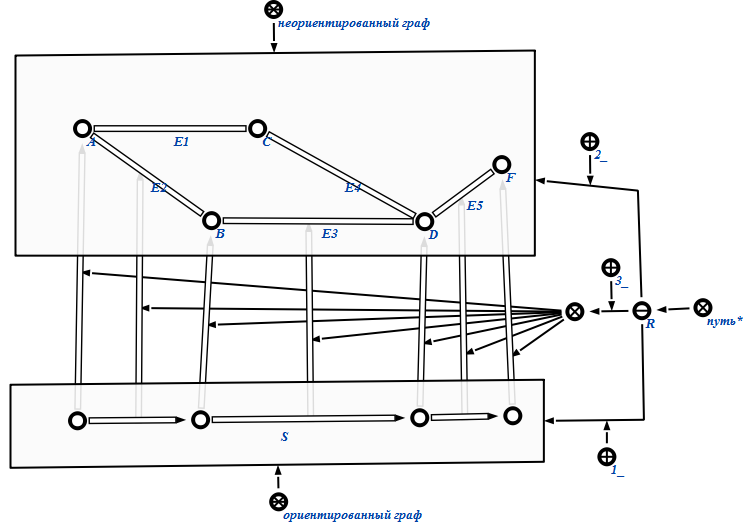
\includegraphics[scale=0.7]{images/16.png}
  \caption{Выход теста 2}
\end{figure}

\subsection{Тест 3}

\textbf{Вход:}

Необходимо найти минимальный путь между вершинами \emph{A} и \emph{K}.

\begin{figure}[H]
  \centering
  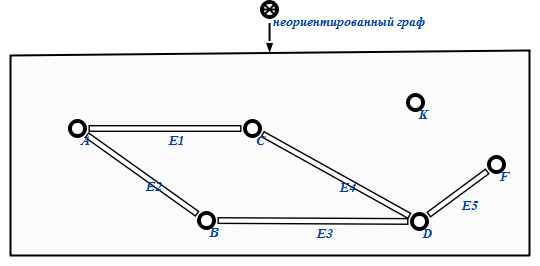
\includegraphics[scale=0.7]{images/17.png}
  \caption{Вход теста 3}
\end{figure}

\textbf{Выход:}

Минимального пути между вершинами \emph{A} и \emph{K} не существует.
Программа должна вернуть ошибку вызывающему контексту.

\subsection{Тест 4}

\textbf{Вход:}

Необходимо найти минимальный путь между вершинами \emph{V5} и
\emph{V11}.

\begin{figure}[H]
  \centering
  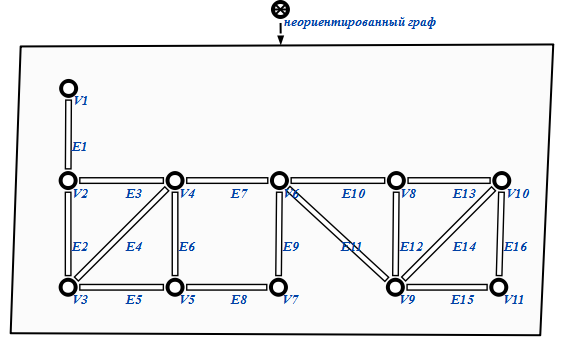
\includegraphics[scale=0.7]{images/18.png}
  \caption{Вход теста 4}
\end{figure}

\textbf{Выход:}

Будет найден один из двух минимальный путь \emph{V5}, \emph{E8},
\emph{V7}, \emph{E9}, \emph{V6}, \emph{E11}, \emph{V9, E15, V11}:

\begin{figure}[H]
  \centering
  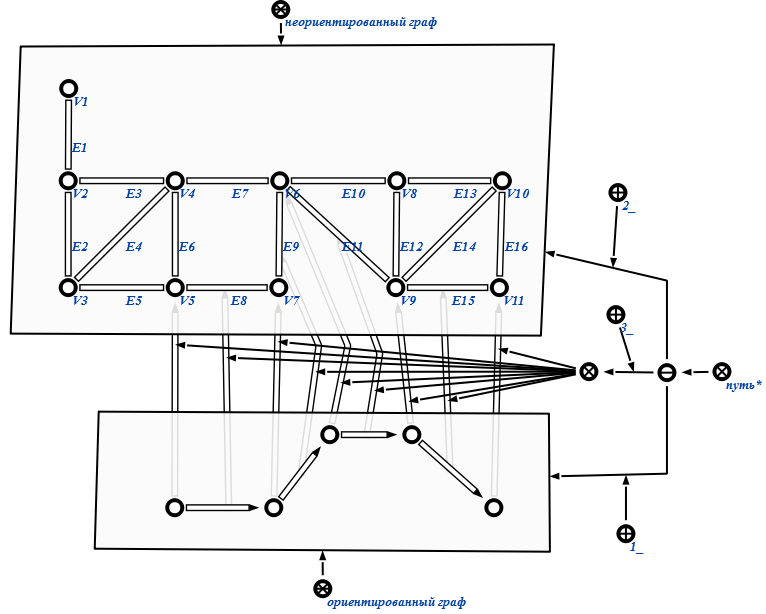
\includegraphics[scale=0.7]{images/19.png}
  \caption{Выход теста 4}
\end{figure}

\subsection{Тест 5}

\textbf{Вход:}

Необходимо найти минимальный путь между вершинами \emph{V1} и \emph{V9}.

\begin{figure}[H]
  \centering
  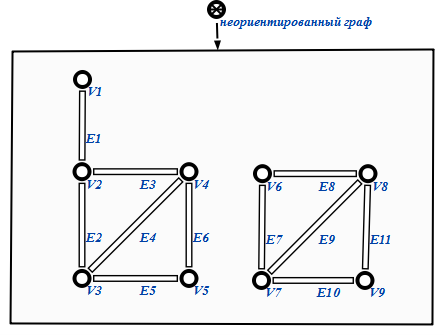
\includegraphics[scale=0.7]{images/20.png}
  \caption{Вход теста 5}
\end{figure}

\textbf{Выход:}

Минимального пути между вершинами \emph{V1} и \emph{V9} не существует. Программа должна вернуть ошибку вызывающему контексту.

\section{Пример работы алгоритма в семантической памяти}

Пример см. в ai\_rr.pdf